\documentclass[mathserif]{beamer}
% Custom definitions
% To use this customization file, insert the line "% Custom definitions
% To use this customization file, insert the line "% Custom definitions
% To use this customization file, insert the line "\input{custom}" in the header of the tex file.

% Formatting

\tolerance=1000
\usepackage[margin=1in]{geometry}


% Packages

% \usepackage{amssymb,latexsym}
\usepackage{amssymb,amsfonts,amsmath,latexsym,amsthm}
%\usepackage[usenames,dvipsnames]{color}
\usepackage[]{graphicx}
\usepackage[space]{grffile}
\usepackage{mathrsfs}   % fancy math font
% \usepackage[font=small,skip=0pt]{caption}
\usepackage[skip=0pt]{caption}
\usepackage{subcaption}
\usepackage{verbatim}
\usepackage{url}
\usepackage{bm}
\usepackage{dsfont}
\usepackage{extarrows}
\usepackage{multirow}
% \usepackage{wrapfig}
% \usepackage{epstopdf}
\usepackage{rotating}
\usepackage{tikz}
\usetikzlibrary{fit}					% fitting shapes to coordinates
%\usetikzlibrary{backgrounds}	% drawing the background after the foreground


% \usepackage[dvipdfm,colorlinks,citecolor=blue,linkcolor=blue,urlcolor=blue]{hyperref}
\usepackage[colorlinks,citecolor=blue,linkcolor=blue,urlcolor=blue]{hyperref}
%\usepackage{hyperref}
\usepackage[authoryear,round]{natbib}


%  Theorems, etc.

\theoremstyle{plain}
\newtheorem{theorem}{Theorem}[section]
\newtheorem{corollary}[theorem]{Corollary}
\newtheorem{lemma}[theorem]{Lemma}
\newtheorem{proposition}[theorem]{Proposition}
\newtheorem{condition}[theorem]{Condition}
% \newtheorem{conditions}[theorem]{Conditions}

\theoremstyle{definition}
\newtheorem{definition}[theorem]{Definition}
% \newtheorem*{unnumbered-definition}{Definition}
\newtheorem{example}[theorem]{Example}
\theoremstyle{remark}
\newtheorem*{remark}{Remark}
\numberwithin{equation}{section}




% Document-specific shortcuts
\newcommand{\btheta}{{\bm\theta}}
\newcommand{\bbtheta}{{\pmb{\bm\theta}}}

\newcommand{\commentary}[1]{\ifx\showcommentary\undefined\else \emph{#1}\fi}

\newcommand{\term}[1]{\textit{\textbf{#1}}}

% Math shortcuts

% Probability distributions
\DeclareMathOperator*{\Exp}{Exp}
\DeclareMathOperator*{\TExp}{TExp}
\DeclareMathOperator*{\Bernoulli}{Bernoulli}
\DeclareMathOperator*{\Beta}{Beta}
\DeclareMathOperator*{\Ga}{Gamma}
\DeclareMathOperator*{\TGamma}{TGamma}
\DeclareMathOperator*{\Poisson}{Poisson}
\DeclareMathOperator*{\Binomial}{Binomial}
\DeclareMathOperator*{\NormalGamma}{NormalGamma}
\DeclareMathOperator*{\InvGamma}{InvGamma}
\DeclareMathOperator*{\Cauchy}{Cauchy}
\DeclareMathOperator*{\Uniform}{Uniform}
\DeclareMathOperator*{\Gumbel}{Gumbel}
\DeclareMathOperator*{\Pareto}{Pareto}
\DeclareMathOperator*{\Mono}{Mono}
\DeclareMathOperator*{\Geometric}{Geometric}
\DeclareMathOperator*{\Wishart}{Wishart}

% Math operators
\DeclareMathOperator*{\argmin}{arg\,min}
\DeclareMathOperator*{\argmax}{arg\,max}
\DeclareMathOperator*{\Cov}{Cov}
\DeclareMathOperator*{\diag}{diag}
\DeclareMathOperator*{\median}{median}
\DeclareMathOperator*{\Vol}{Vol}

% Math characters
\newcommand{\R}{\mathbb{R}}
\newcommand{\Z}{\mathbb{Z}}
\newcommand{\E}{\mathbb{E}}
\renewcommand{\Pr}{\mathbb{P}}
\newcommand{\I}{\mathds{1}}
\newcommand{\V}{\mathbb{V}}

\newcommand{\A}{\mathcal{A}}
\newcommand{\C}{\mathcal{C}}
\newcommand{\D}{\mathcal{D}}
\newcommand{\Hcal}{\mathcal{H}}
\newcommand{\M}{\mathcal{M}}
\newcommand{\N}{\mathcal{N}}
\newcommand{\X}{\mathcal{X}}
\newcommand{\Zcal}{\mathcal{Z}}
\renewcommand{\P}{\mathcal{P}}

\newcommand{\T}{\mathtt{T}}
\renewcommand{\emptyset}{\varnothing}


% Miscellaneous commands
\newcommand{\iid}{\stackrel{\mathrm{iid}}{\sim}}
\newcommand{\matrixsmall}[1]{\bigl(\begin{smallmatrix}#1\end{smallmatrix} \bigr)}

\newcommand{\items}[1]{\begin{itemize} #1 \end{itemize}}

\newcommand{\todo}[1]{\emph{\textcolor{red}{(#1)}}}

\newcommand{\branch}[4]{
\left\{
	\begin{array}{ll}
		#1  & \mbox{if } #2 \\
		#3 & \mbox{if } #4
	\end{array}
\right.
}

% approximately proportional to
\def\app#1#2{%
  \mathrel{%
    \setbox0=\hbox{$#1\sim$}%
    \setbox2=\hbox{%
      \rlap{\hbox{$#1\propto$}}%
      \lower1.3\ht0\box0%
    }%
    \raise0.25\ht2\box2%
  }%
}
\def\approxprop{\mathpalette\app\relax}

% \newcommand{\approptoinn}[2]{\mathrel{\vcenter{
  % \offinterlineskip\halign{\hfil$##$\cr
    % #1\propto\cr\noalign{\kern2pt}#1\sim\cr\noalign{\kern-2pt}}}}}

% \newcommand{\approxpropto}{\mathpalette\approptoinn\relax}





" in the header of the tex file.

% Formatting

\tolerance=1000
\usepackage[margin=1in]{geometry}


% Packages

% \usepackage{amssymb,latexsym}
\usepackage{amssymb,amsfonts,amsmath,latexsym,amsthm}
%\usepackage[usenames,dvipsnames]{color}
\usepackage[]{graphicx}
\usepackage[space]{grffile}
\usepackage{mathrsfs}   % fancy math font
% \usepackage[font=small,skip=0pt]{caption}
\usepackage[skip=0pt]{caption}
\usepackage{subcaption}
\usepackage{verbatim}
\usepackage{url}
\usepackage{bm}
\usepackage{dsfont}
\usepackage{extarrows}
\usepackage{multirow}
% \usepackage{wrapfig}
% \usepackage{epstopdf}
\usepackage{rotating}
\usepackage{tikz}
\usetikzlibrary{fit}					% fitting shapes to coordinates
%\usetikzlibrary{backgrounds}	% drawing the background after the foreground


% \usepackage[dvipdfm,colorlinks,citecolor=blue,linkcolor=blue,urlcolor=blue]{hyperref}
\usepackage[colorlinks,citecolor=blue,linkcolor=blue,urlcolor=blue]{hyperref}
%\usepackage{hyperref}
\usepackage[authoryear,round]{natbib}


%  Theorems, etc.

\theoremstyle{plain}
\newtheorem{theorem}{Theorem}[section]
\newtheorem{corollary}[theorem]{Corollary}
\newtheorem{lemma}[theorem]{Lemma}
\newtheorem{proposition}[theorem]{Proposition}
\newtheorem{condition}[theorem]{Condition}
% \newtheorem{conditions}[theorem]{Conditions}

\theoremstyle{definition}
\newtheorem{definition}[theorem]{Definition}
% \newtheorem*{unnumbered-definition}{Definition}
\newtheorem{example}[theorem]{Example}
\theoremstyle{remark}
\newtheorem*{remark}{Remark}
\numberwithin{equation}{section}




% Document-specific shortcuts
\newcommand{\btheta}{{\bm\theta}}
\newcommand{\bbtheta}{{\pmb{\bm\theta}}}

\newcommand{\commentary}[1]{\ifx\showcommentary\undefined\else \emph{#1}\fi}

\newcommand{\term}[1]{\textit{\textbf{#1}}}

% Math shortcuts

% Probability distributions
\DeclareMathOperator*{\Exp}{Exp}
\DeclareMathOperator*{\TExp}{TExp}
\DeclareMathOperator*{\Bernoulli}{Bernoulli}
\DeclareMathOperator*{\Beta}{Beta}
\DeclareMathOperator*{\Ga}{Gamma}
\DeclareMathOperator*{\TGamma}{TGamma}
\DeclareMathOperator*{\Poisson}{Poisson}
\DeclareMathOperator*{\Binomial}{Binomial}
\DeclareMathOperator*{\NormalGamma}{NormalGamma}
\DeclareMathOperator*{\InvGamma}{InvGamma}
\DeclareMathOperator*{\Cauchy}{Cauchy}
\DeclareMathOperator*{\Uniform}{Uniform}
\DeclareMathOperator*{\Gumbel}{Gumbel}
\DeclareMathOperator*{\Pareto}{Pareto}
\DeclareMathOperator*{\Mono}{Mono}
\DeclareMathOperator*{\Geometric}{Geometric}
\DeclareMathOperator*{\Wishart}{Wishart}

% Math operators
\DeclareMathOperator*{\argmin}{arg\,min}
\DeclareMathOperator*{\argmax}{arg\,max}
\DeclareMathOperator*{\Cov}{Cov}
\DeclareMathOperator*{\diag}{diag}
\DeclareMathOperator*{\median}{median}
\DeclareMathOperator*{\Vol}{Vol}

% Math characters
\newcommand{\R}{\mathbb{R}}
\newcommand{\Z}{\mathbb{Z}}
\newcommand{\E}{\mathbb{E}}
\renewcommand{\Pr}{\mathbb{P}}
\newcommand{\I}{\mathds{1}}
\newcommand{\V}{\mathbb{V}}

\newcommand{\A}{\mathcal{A}}
\newcommand{\C}{\mathcal{C}}
\newcommand{\D}{\mathcal{D}}
\newcommand{\Hcal}{\mathcal{H}}
\newcommand{\M}{\mathcal{M}}
\newcommand{\N}{\mathcal{N}}
\newcommand{\X}{\mathcal{X}}
\newcommand{\Zcal}{\mathcal{Z}}
\renewcommand{\P}{\mathcal{P}}

\newcommand{\T}{\mathtt{T}}
\renewcommand{\emptyset}{\varnothing}


% Miscellaneous commands
\newcommand{\iid}{\stackrel{\mathrm{iid}}{\sim}}
\newcommand{\matrixsmall}[1]{\bigl(\begin{smallmatrix}#1\end{smallmatrix} \bigr)}

\newcommand{\items}[1]{\begin{itemize} #1 \end{itemize}}

\newcommand{\todo}[1]{\emph{\textcolor{red}{(#1)}}}

\newcommand{\branch}[4]{
\left\{
	\begin{array}{ll}
		#1  & \mbox{if } #2 \\
		#3 & \mbox{if } #4
	\end{array}
\right.
}

% approximately proportional to
\def\app#1#2{%
  \mathrel{%
    \setbox0=\hbox{$#1\sim$}%
    \setbox2=\hbox{%
      \rlap{\hbox{$#1\propto$}}%
      \lower1.3\ht0\box0%
    }%
    \raise0.25\ht2\box2%
  }%
}
\def\approxprop{\mathpalette\app\relax}

% \newcommand{\approptoinn}[2]{\mathrel{\vcenter{
  % \offinterlineskip\halign{\hfil$##$\cr
    % #1\propto\cr\noalign{\kern2pt}#1\sim\cr\noalign{\kern-2pt}}}}}

% \newcommand{\approxpropto}{\mathpalette\approptoinn\relax}





" in the header of the tex file.

% Formatting

\tolerance=1000
\usepackage[margin=1in]{geometry}


% Packages

% \usepackage{amssymb,latexsym}
\usepackage{amssymb,amsfonts,amsmath,latexsym,amsthm}
%\usepackage[usenames,dvipsnames]{color}
\usepackage[]{graphicx}
\usepackage[space]{grffile}
\usepackage{mathrsfs}   % fancy math font
% \usepackage[font=small,skip=0pt]{caption}
\usepackage[skip=0pt]{caption}
\usepackage{subcaption}
\usepackage{verbatim}
\usepackage{url}
\usepackage{bm}
\usepackage{dsfont}
\usepackage{extarrows}
\usepackage{multirow}
% \usepackage{wrapfig}
% \usepackage{epstopdf}
\usepackage{rotating}
\usepackage{tikz}
\usetikzlibrary{fit}					% fitting shapes to coordinates
%\usetikzlibrary{backgrounds}	% drawing the background after the foreground


% \usepackage[dvipdfm,colorlinks,citecolor=blue,linkcolor=blue,urlcolor=blue]{hyperref}
\usepackage[colorlinks,citecolor=blue,linkcolor=blue,urlcolor=blue]{hyperref}
%\usepackage{hyperref}
\usepackage[authoryear,round]{natbib}


%  Theorems, etc.

\theoremstyle{plain}
\newtheorem{theorem}{Theorem}[section]
\newtheorem{corollary}[theorem]{Corollary}
\newtheorem{lemma}[theorem]{Lemma}
\newtheorem{proposition}[theorem]{Proposition}
\newtheorem{condition}[theorem]{Condition}
% \newtheorem{conditions}[theorem]{Conditions}

\theoremstyle{definition}
\newtheorem{definition}[theorem]{Definition}
% \newtheorem*{unnumbered-definition}{Definition}
\newtheorem{example}[theorem]{Example}
\theoremstyle{remark}
\newtheorem*{remark}{Remark}
\numberwithin{equation}{section}




% Document-specific shortcuts
\newcommand{\btheta}{{\bm\theta}}
\newcommand{\bbtheta}{{\pmb{\bm\theta}}}

\newcommand{\commentary}[1]{\ifx\showcommentary\undefined\else \emph{#1}\fi}

\newcommand{\term}[1]{\textit{\textbf{#1}}}

% Math shortcuts

% Probability distributions
\DeclareMathOperator*{\Exp}{Exp}
\DeclareMathOperator*{\TExp}{TExp}
\DeclareMathOperator*{\Bernoulli}{Bernoulli}
\DeclareMathOperator*{\Beta}{Beta}
\DeclareMathOperator*{\Ga}{Gamma}
\DeclareMathOperator*{\TGamma}{TGamma}
\DeclareMathOperator*{\Poisson}{Poisson}
\DeclareMathOperator*{\Binomial}{Binomial}
\DeclareMathOperator*{\NormalGamma}{NormalGamma}
\DeclareMathOperator*{\InvGamma}{InvGamma}
\DeclareMathOperator*{\Cauchy}{Cauchy}
\DeclareMathOperator*{\Uniform}{Uniform}
\DeclareMathOperator*{\Gumbel}{Gumbel}
\DeclareMathOperator*{\Pareto}{Pareto}
\DeclareMathOperator*{\Mono}{Mono}
\DeclareMathOperator*{\Geometric}{Geometric}
\DeclareMathOperator*{\Wishart}{Wishart}

% Math operators
\DeclareMathOperator*{\argmin}{arg\,min}
\DeclareMathOperator*{\argmax}{arg\,max}
\DeclareMathOperator*{\Cov}{Cov}
\DeclareMathOperator*{\diag}{diag}
\DeclareMathOperator*{\median}{median}
\DeclareMathOperator*{\Vol}{Vol}

% Math characters
\newcommand{\R}{\mathbb{R}}
\newcommand{\Z}{\mathbb{Z}}
\newcommand{\E}{\mathbb{E}}
\renewcommand{\Pr}{\mathbb{P}}
\newcommand{\I}{\mathds{1}}
\newcommand{\V}{\mathbb{V}}

\newcommand{\A}{\mathcal{A}}
\newcommand{\C}{\mathcal{C}}
\newcommand{\D}{\mathcal{D}}
\newcommand{\Hcal}{\mathcal{H}}
\newcommand{\M}{\mathcal{M}}
\newcommand{\N}{\mathcal{N}}
\newcommand{\X}{\mathcal{X}}
\newcommand{\Zcal}{\mathcal{Z}}
\renewcommand{\P}{\mathcal{P}}

\newcommand{\T}{\mathtt{T}}
\renewcommand{\emptyset}{\varnothing}


% Miscellaneous commands
\newcommand{\iid}{\stackrel{\mathrm{iid}}{\sim}}
\newcommand{\matrixsmall}[1]{\bigl(\begin{smallmatrix}#1\end{smallmatrix} \bigr)}

\newcommand{\items}[1]{\begin{itemize} #1 \end{itemize}}

\newcommand{\todo}[1]{\emph{\textcolor{red}{(#1)}}}

\newcommand{\branch}[4]{
\left\{
	\begin{array}{ll}
		#1  & \mbox{if } #2 \\
		#3 & \mbox{if } #4
	\end{array}
\right.
}

% approximately proportional to
\def\app#1#2{%
  \mathrel{%
    \setbox0=\hbox{$#1\sim$}%
    \setbox2=\hbox{%
      \rlap{\hbox{$#1\propto$}}%
      \lower1.3\ht0\box0%
    }%
    \raise0.25\ht2\box2%
  }%
}
\def\approxprop{\mathpalette\app\relax}

% \newcommand{\approptoinn}[2]{\mathrel{\vcenter{
  % \offinterlineskip\halign{\hfil$##$\cr
    % #1\propto\cr\noalign{\kern2pt}#1\sim\cr\noalign{\kern-2pt}}}}}

% \newcommand{\approxpropto}{\mathpalette\approptoinn\relax}






\setbeamertemplate{frametitle}[default][center]%Centers the frame title.
\setbeamertemplate{navigation symbols}{}%Removes navigation symbols.
\setbeamertemplate{footline}{\raisebox{5pt}{\makebox[\paperwidth]{\hfill\makebox[10pt]{\scriptsize\insertframenumber}}}}
\setbeamertemplate{caption}[numbered]

\usepackage{amssymb,amsfonts,amsmath,latexsym,amsthm}
%\usepackage[usenames,dvipsnames]{color}
%\usepackage[]{graphicx}
%\usepackage[space]{grffile}
\usepackage{mathrsfs}   % fancy math font
% \usepackage[font=small,skip=0pt]{caption}
\usepackage[skip=0pt]{caption}
\usepackage{subcaption}
\usepackage{verbatim}
\usepackage{url}
\usepackage{bm}
\usepackage{dsfont}
\usepackage{extarrows}
\usepackage{multirow, bm}
%\newcommand{\tth}   {\mbox{$\theta$}}
\newcommand{\thh}   {\mbox{$\theta$}}
\newcommand{\su}   {\mbox{$\sigma^2$}}
\newcommand{\so}   {\mbox{$\sigma_0^2$}}
\newcommand{\ko}   {\mbox{$\kappa_0$}}
\newcommand{\no}   {\mbox{$\nu_0$}}
\newcommand{\mo}   {\mbox{$\mu_0$}}
\newcommand{\ti}   {\mbox{$\tilde{x}$}}
\newcommand{\la}   {\mbox{$\lambda$}}
\newcommand{\bx}   {\mbox{$\bm{x}$}}
\newcommand{\bZ}   {\mbox{$\bm{Z}$}}
\newcommand{\bX}   {\mbox{$\bm{X}$}}
\newcommand{\bY}   {\mbox{$\bm{Y}$}}
\newcommand{\bA}   {\mbox{$\bm{A}$}}
\newcommand{\ba}   {\mbox{$\bm{a}$}}
\newcommand{\bb}   {\mbox{$\bm{b}$}}
\newcommand{\bt}   {\mbox{$\bm{t}$}}
\newcommand{\bz}   {\mbox{$\bm{z}$}}
\newcommand{\bw}   {\mbox{$\bm{w}$}}
\newcommand{\bbeta}   {\mbox{$\bm{\beta}$}}

\newcommand{\be}   {\mbox{$\bm{e}$}}
\newcommand{\bu}   {\mbox{$\bm{u}$}}
\newcommand{\bv}   {\mbox{$\bm{v}$}}
\newcommand{\sig}   {\mbox{$\Sigma$}}
\newcommand{\sigx}   {\mbox{$\Sigma_{XX}$}}
\newcommand{\sigxy}   {\mbox{$\Sigma_{XY}$}}
\newcommand{\tr}   {\mbox{$\text{tr}$}}
\newcommand{\ddet}   {\mbox{$\text{det}$}}
\newcommand\independent{\protect\mathpalette{\protect\independenT}{\perp}}
\def\independenT#1#2{\mathrel{\rlap{$#1#2$}\mkern2mu{#1#2}}}

\newcommand{\Expect}[1]{\ensuremath{\mathbf{E}\left[ #1 \right]}}
%\newcommand{\Var}[1]{\ensuremath{\mathrm{Var}\left[ #1 \right]}}
%\newcommand{\Cov}[1]{\ensuremath{\mathrm{Cov}\left[ #1 \right]}}
\newcommand{\MSE}{\ensuremath{\mathrm{MSE}}}
\newcommand{\RSS}{\ensuremath{\mathrm{RSS}}}
\newcommand{\Prob}[1]{\ensuremath{\mathrm{Pr}\left( #1 \right)}}
\newcommand{\ProbEst}[1]{\ensuremath{\widehat{\mathrm{Pr}}\left( #1 \right)}}
\DeclareMathOperator*{\argmin}{argmin} % thanks, wikipedia!
\DeclareMathOperator*{\argmax}{argmax} % thanks, wikipedia!
\DeclareMathOperator*{\sgn}{sgn} % thanks, wikipedia!

\newcommand{\lam}{\lambda}
\newcommand{\bmu}{\bm{\mu}}
%\newcommand{\bx}{\ensuremath{\mathbf{X}}}
\newcommand{\X}{\ensuremath{\mathbf{X}}}
\newcommand{\w}{\ensuremath{\mathbf{w}}}
\newcommand{\h}{\ensuremath{\mathbf{h}}}
\newcommand{\V}{\ensuremath{\mathbf{V}}}
%\newcommand{\tr}{\operatorname{tr}}

%\newcommand{\bx}{\ensuremath{\mathbf{X}}}
%\newcommand{\X}{\ensuremath{\mathbf{x}}}
%\newcommand{\w}{\ensuremath{\mathbf{w}}}
%\newcommand{\h}{\ensuremath{\mathbf{h}}}
%\newcommand{\V}{\ensuremath{\mathbf{v}}}
%\newcommand{\Cov}{\text{Cov}}
%\newcommand{\Var}{\text{Var}}

\DeclareMathOperator{\var}{Var}
\DeclareMathOperator{\cov}{Cov}
\newcommand{\Var}[1]{\ensuremath{\mathrm{Var}\left[ #1 \right]}}
\newcommand{\Cov}[1]{\ensuremath{\mathrm{Cov}\left[ #1 \right]}}


\newcommand{\indep}{\rotatebox{90}{\ensuremath{\models}}}
\newcommand{\notindep}{\not\hspace{-.05in}\indep}








\usepackage{float,bm}
\floatstyle{boxed}
\newfloat{code}{tp}{code}
\floatname{code}{Code Example}
%\newcommand{\tth}   {\mbox{$\theta$}}
\newcommand{\thh}   {\mbox{$\theta$}}
\newcommand{\su}   {\mbox{$\sigma^2$}}
\newcommand{\so}   {\mbox{$\sigma_0^2$}}
\newcommand{\ko}   {\mbox{$\kappa_0$}}
\newcommand{\no}   {\mbox{$\nu_0$}}
\newcommand{\mo}   {\mbox{$\mu_0$}}
\newcommand{\ti}   {\mbox{$\tilde{x}$}}
\newcommand{\la}   {\mbox{$\lambda$}}
\newcommand{\bx}   {\mbox{$\bm{x}$}}
\newcommand{\bZ}   {\mbox{$\bm{Z}$}}
\newcommand{\bX}   {\mbox{$\bm{X}$}}
\newcommand{\bY}   {\mbox{$\bm{Y}$}}
\newcommand{\bA}   {\mbox{$\bm{A}$}}
\newcommand{\ba}   {\mbox{$\bm{a}$}}
\newcommand{\bb}   {\mbox{$\bm{b}$}}
\newcommand{\bt}   {\mbox{$\bm{t}$}}
\newcommand{\bz}   {\mbox{$\bm{z}$}}
\newcommand{\bw}   {\mbox{$\bm{w}$}}
\newcommand{\bbeta}   {\mbox{$\bm{\beta}$}}

\newcommand{\be}   {\mbox{$\bm{e}$}}
\newcommand{\bu}   {\mbox{$\bm{u}$}}
\newcommand{\bv}   {\mbox{$\bm{v}$}}
\newcommand{\sig}   {\mbox{$\Sigma$}}
\newcommand{\sigx}   {\mbox{$\Sigma_{XX}$}}
\newcommand{\sigxy}   {\mbox{$\Sigma_{XY}$}}
\newcommand{\tr}   {\mbox{$\text{tr}$}}
\newcommand{\ddet}   {\mbox{$\text{det}$}}
\newcommand\independent{\protect\mathpalette{\protect\independenT}{\perp}}
\def\independenT#1#2{\mathrel{\rlap{$#1#2$}\mkern2mu{#1#2}}}

\newcommand{\Expect}[1]{\ensuremath{\mathbf{E}\left[ #1 \right]}}
%\newcommand{\Var}[1]{\ensuremath{\mathrm{Var}\left[ #1 \right]}}
%\newcommand{\Cov}[1]{\ensuremath{\mathrm{Cov}\left[ #1 \right]}}
\newcommand{\MSE}{\ensuremath{\mathrm{MSE}}}
\newcommand{\RSS}{\ensuremath{\mathrm{RSS}}}
\newcommand{\Prob}[1]{\ensuremath{\mathrm{Pr}\left( #1 \right)}}
\newcommand{\ProbEst}[1]{\ensuremath{\widehat{\mathrm{Pr}}\left( #1 \right)}}
\DeclareMathOperator*{\argmin}{argmin} % thanks, wikipedia!
\DeclareMathOperator*{\argmax}{argmax} % thanks, wikipedia!
\DeclareMathOperator*{\sgn}{sgn} % thanks, wikipedia!

\newcommand{\lam}{\lambda}
\newcommand{\bmu}{\bm{\mu}}
%\newcommand{\bx}{\ensuremath{\mathbf{X}}}
\newcommand{\X}{\ensuremath{\mathbf{X}}}
\newcommand{\w}{\ensuremath{\mathbf{w}}}
\newcommand{\h}{\ensuremath{\mathbf{h}}}
\newcommand{\V}{\ensuremath{\mathbf{V}}}
%\newcommand{\tr}{\operatorname{tr}}

%\newcommand{\bx}{\ensuremath{\mathbf{X}}}
%\newcommand{\X}{\ensuremath{\mathbf{x}}}
%\newcommand{\w}{\ensuremath{\mathbf{w}}}
%\newcommand{\h}{\ensuremath{\mathbf{h}}}
%\newcommand{\V}{\ensuremath{\mathbf{v}}}
%\newcommand{\Cov}{\text{Cov}}
%\newcommand{\Var}{\text{Var}}

\DeclareMathOperator{\var}{Var}
\DeclareMathOperator{\cov}{Cov}
\newcommand{\Var}[1]{\ensuremath{\mathrm{Var}\left[ #1 \right]}}
\newcommand{\Cov}[1]{\ensuremath{\mathrm{Cov}\left[ #1 \right]}}


\newcommand{\indep}{\rotatebox{90}{\ensuremath{\models}}}
\newcommand{\notindep}{\not\hspace{-.05in}\indep}






%\usepackage{fontspec}
%\setmainfont{Tahoma}

%\newcommand{\lam}{\alpha}
\newcommand{\bmu}{\bm{\mu}}
\newcommand{\bX}   {\bm{X}}
\newcommand{\sig}   {\Sigma}
\newcommand{\bx}{\ensuremath{\mathbf{X}}}
%\newcommand{\X}{\ensuremath{\mathbf{x}}}
%\newcommand{\w}{\ensuremath{\mathbf{w}}}
%\newcommand{\h}{\ensuremath{\mathbf{h}}}
%\newcommand{\V}{\ensuremath{\mathbf{v}}}
%\newcommand{\cov}{\text{Cov}}
\newcommand{\var}{\text{Var}}

%\DeclareMathOperator{\var}{Var}
%\DeclareMathOperator{\cov}{Cov}

%\newcommand{\indep}{\rotatebox{90}{\ensuremath{\models}}}
%\newcommand{\notindep}{\not\hspace{-.05in}\indep}



\newcommand{\beginbackup}{
   \newcounter{framenumbervorappendix}
   \setcounter{framenumbervorappendix}{\value{framenumber}}
}
\newcommand{\backupend}{
   \addtocounter{framenumbervorappendix}{-\value{framenumber}}
   \addtocounter{framenumber}{\value{framenumbervorappendix}} 
}


%\usepackage{algorithm2e}
\usepackage[ruled,lined]{algorithm2e}
\def\algorithmautorefname{Algorithm}
\SetKwIF{If}{ElseIf}{Else}{if}{then}{else if}{else}{endif}
%\usepackage{times}
%\usepackage[tbtags]{amsmath}
%\usepackage{amssymb}
\usepackage{amsfonts}
%\usepackage{slfortheorems}
\usepackage{epsfig}
\usepackage{graphicx}
%\usepackage[small]{caption}
%\usepackage[square]{natbib}
%\newcommand{\newblock}{}
%\bibpunct{(}{)}{;}{a}{}{,}
%\bibliographystyle{ims}
%\usepackage[letterpaper]{geometry}
%\usepackage{color}
%\setlength{\parindent}{0pt}

\usepackage{natbib}
\bibpunct{(}{)}{;}{a}{}{,}
%\usepackage{hyperref}

%\DeclareMathOperator*{\Exp}{Exp}
%\DeclareMathOperator*{\TExp}{TExp}
%\DeclareMathOperator*{\Bernoulli}{Bernoulli}
%\DeclareMathOperator*{\Beta}{Beta}
%\DeclareMathOperator*{\Ga}{Gamma}
%\DeclareMathOperator*{\TGamma}{TGamma}
%\DeclareMathOperator*{\Poisson}{Poisson}
%\DeclareMathOperator*{\Binomial}{Binomial}
%\DeclareMathOperator*{\NormalGamma}{NormalGamma}
%\DeclareMathOperator*{\InvGamma}{InvGamma}
%\DeclareMathOperator*{\Cauchy}{Cauchy}
%\DeclareMathOperator*{\Uniform}{Uniform}
%\DeclareMathOperator*{\Gumbel}{Gumbel}
%\DeclareMathOperator*{\Pareto}{Pareto}
%\DeclareMathOperator*{\Mono}{Mono}
%\DeclareMathOperator*{\Geometric}{Geometric}
%\DeclareMathOperator*{\Wishart}{Wishart}

%\newcommand{\N}{\mathcal{N}}
%
%\newcommand{\R}{\mathbb{R}}
%\newcommand{\Z}{\mathbb{Z}}
%\newcommand{\E}{\mathbb{E}}
%\renewcommand{\Pr}{\mathbb{P}}
%\newcommand{\I}{\mathds{1}}
%\newcommand{\V}{\mathbb{V}}

%% Math operators
%\DeclareMathOperator*{\diag}{diag}
%\DeclareMathOperator*{\median}{median}
%\DeclareMathOperator*{\Vol}{Vol}
%
%% Miscellaneous commands
%\newcommand{\iid}{\stackrel{\mathrm{iid}}{\sim}}
%\newcommand{\matrixsmall}[1]{\bigl(\begin{smallmatrix}#1\end{smallmatrix} \bigr)}
%
%\newcommand{\items}[1]{\begin{itemize} #1 \end{itemize}}
%
%\newcommand{\todo}[1]{\emph{\textcolor{red}{(#1)}}}
%
%\newcommand{\branch}[4]{
%\left\{
%	\begin{array}{ll}
%		#1  & \mbox{if } #2 \\
%		#3 & \mbox{if } #4
%	\end{array}
%\right.
%}
%
%% approximately proportional to
%\def\app#1#2{%
%  \mathrel{%
%    \setbox0=\hbox{$#1\sim$}%
%    \setbox2=\hbox{%
%      \rlap{\hbox{$#1\propto$}}%
%      \lower1.3\ht0\box0%
%    }%
%    \raise0.25\ht2\box2%
%  }%
%}
%\def\approxprop{\mathpalette\app\relax}
%
%\newcommand{\btheta}{{\bm\theta}}
%\newcommand{\bbtheta}{{\pmb{\bm\theta}}}

%\usepackage{zref-savepos}
%
%\newcounter{restofframe}
%\newsavebox{\restofframebox}
%\newlength{\mylowermargin}
%\setlength{\mylowermargin}{2pt}
%
%\newenvironment{restofframe}{%
%    \par%\centering
%    \stepcounter{restofframe}%
%    \zsavepos{restofframe-\arabic{restofframe}-begin}%
%    \begin{lrbox}{\restofframebox}%
%}{%
%    \end{lrbox}%
%    \setkeys{Gin}{keepaspectratio}%
%    \raisebox{\dimexpr-\height+\ht\strutbox\relax}[0pt][0pt]{%
%    \resizebox*{!}{\dimexpr\zposy{restofframe-\arabic{restofframe}-begin}sp-\zposy{restofframe-\arabic{restofframe}-end}sp-\mylowermargin\relax}%
%        {\usebox{\restofframebox}}%
%    }%
%    \vskip0pt plus 1filll\relax
%    \mbox{\zsavepos{restofframe-\arabic{restofframe}-end}}%
%    \par
%}


\usepackage{tikz}
\usetikzlibrary{arrows}

%\usepackage[usenames,dvipsnames]{xcolor}
\usepackage{tkz-berge}
\usetikzlibrary{fit,shapes}

\usepackage{calc}
%%
%% The tikz package is used for doing the actual drawing.
%\usepackage{tikz}
%%
%% In order to be able to put arrowheads in the middle of directed edges, we need an extra library.
\usetikzlibrary{decorations.markings}
%%
%% The next line says how the "vertex" style of nodes should look: drawn as small circles.
\tikzstyle{vertex}=[circle, draw, inner sep=0pt, minimum size=6pt]
%%
%% Next, we make a \vertex command as a shorthand in place of \node[vertex} to get that style.
\newcommand{\vertex}{\node[vertex]}
%%
%% Finally, we declare a "counter", which is what LaTeX calls an integer variable, for use in
%% the calculations of angles for evenly spacing vertices in circular arrangements.
\newcounter{Angle}

\newtheoremstyle{example}
{\topsep} % space above
{\topsep} % space below
{} % body font
{} % indent
{\bf} % head font
{:} % punctuation between head and body
{0.5em} % space after head
{} % manually specify head
%{\thmname{#1}\thmnumber{ #2}\thmnote{:#3}} % manually specify head

\theoremstyle{example}
\newtheorem{ex}{Example}[section]

\newtheoremstyle{definition}
{\topsep} % space above
{\topsep} % space below
{} % body font
{} % indent
{\sc} % head font
{:} % punctuation between head and body
{0.5em} % space after head
{} % manually specify head
%{\thmname{#1}\thmnumber{ #2}\thmnote{:#3}} % manually specify head

\theoremstyle{definition}
\newtheorem{defn}{Definition}[section]

\theoremstyle{rem}
\newtheorem{rem}{Remark}[section]

\newtheoremstyle{theorem}
{\topsep} % space above
{\topsep} % space below
{} % body font
{} % indent
{\sc} % head font
{:} % punctuation between head and body
{0.5em} % space after head
{} % manually specify head
%{\thmname{#1}\thmnumber{ #2}\thmnote{:#3}} % manually specify head

\theoremstyle{theorm}
\newtheorem{thm}{Theorem}[section]



%%%to add in new counter for slides in beamer

%\setbeamertemplate{footline}{
%  \leavevmode%
%  \hbox{%
%  \begin{beamercolorbox}[wd=.333333\paperwidth,ht=2.25ex,dp=1ex,center]{author in head/foot}%
%    \usebeamerfont{author in head/foot}\insertshortauthor~~(\insertshortinstitute)
%  \end{beamercolorbox}%
%  \begin{beamercolorbox}[wd=.333333\paperwidth,ht=2.25ex,dp=1ex,center]{title in head/foot}%
%    \usebeamerfont{title in head/foot}\insertshorttitle
%  \end{beamercolorbox}%
%  \begin{beamercolorbox}[wd=.333333\paperwidth,ht=2.25ex,dp=1ex,right]{date in head/foot}%
%    \usebeamerfont{date in head/foot}\insertshortdate{}\hspace*{2em}
%    \insertframenumber{} \hspace*{2ex} % hier hat's sich ge�ndert
%  \end{beamercolorbox}}%
%  \vskip0pt%
%}



%%%%%

\newcommand*\oldmacro{}
\let\oldmacro\insertshortauthor
\renewcommand*\insertshortauthor{
  \leftskip=.3cm
\insertframenumber\,/\,\inserttotalframenumber\hfill\oldmacro}




%\excludecomment{notbeamer}
%\includecomment{beamer}



\title{An Introduction to Bayesian Nonparametric Methods}
\author{Rebecca C. Steorts \\ Bayesian Methods and Modern Statistics: STA 360/601}
\date{Module 11}

\begin{document}

\maketitle

%\frame{
%\frametitle{Bayesian Nonparametric (BNP) Motivation}
%\begin{figure}[htbp]
%\begin{center}
%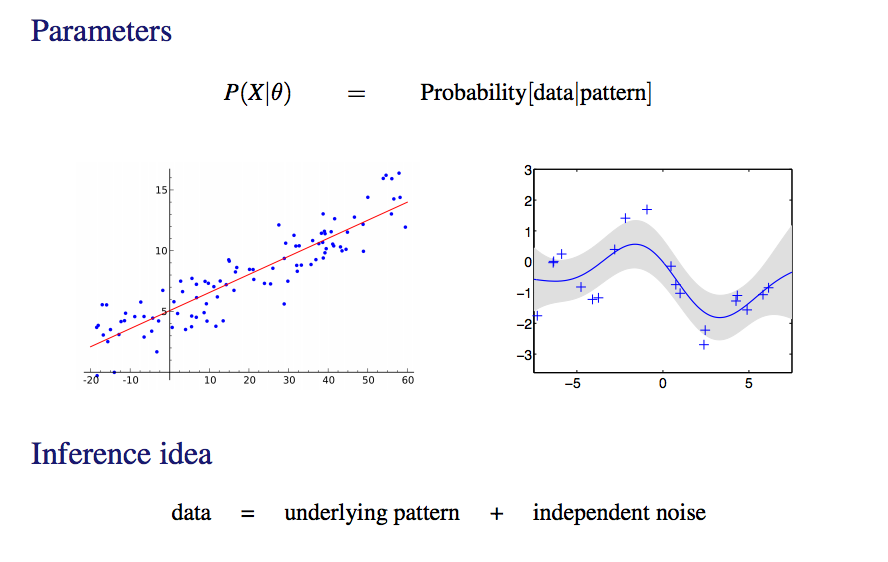
\includegraphics[width=0.9\textwidth]{beingBayesian}
%\label{default}
%\end{center}
%\end{figure}
%
%[Picture: Peter Orbanz, Columbia University]
%
%}

\frame{
\frametitle{What is a nonparametric model?}

\begin{enumerate}
\item A really large parametric model.
\item A parametric model where the number of parameters increases with data.
\item A family of distributions that is dense in some large space relevant to the problem at hand.
\end{enumerate}

}

\frame{
\frametitle{What is NOT a nonparametric model?}

Gaussian model. 

\begin{align}
X \mid \mu &\sim N(\mu,\sigma^2)\\
\mu &\sim N(\mu_o, \tau^2)
\end{align}

Why is this parametric? 

\vskip 1em

Why is it NOT an NP model? 

}

\frame{
\frametitle{Bayesian Nonparametrics}

\begin{figure}[htbp]
\begin{center}
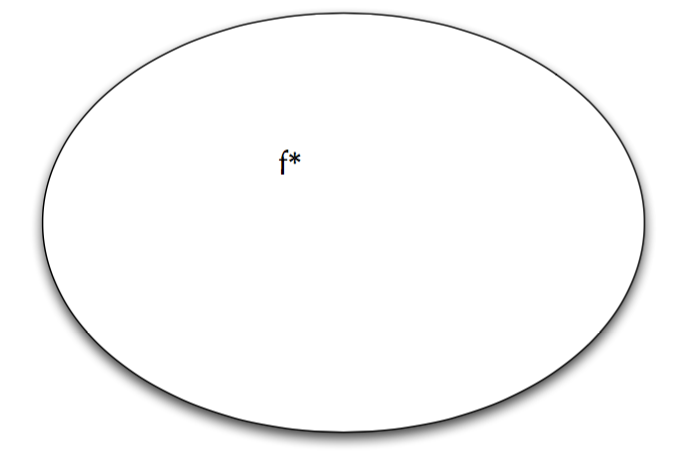
\includegraphics[width=0.8\textwidth]{f}
\label{default}
\end{center}
\end{figure}

Let's do classification. Have inputs and outputs (binary). What is the true output?

}

\frame{
\frametitle{Bayesian Nonparametrics}

\begin{figure}[htbp]
\begin{center}
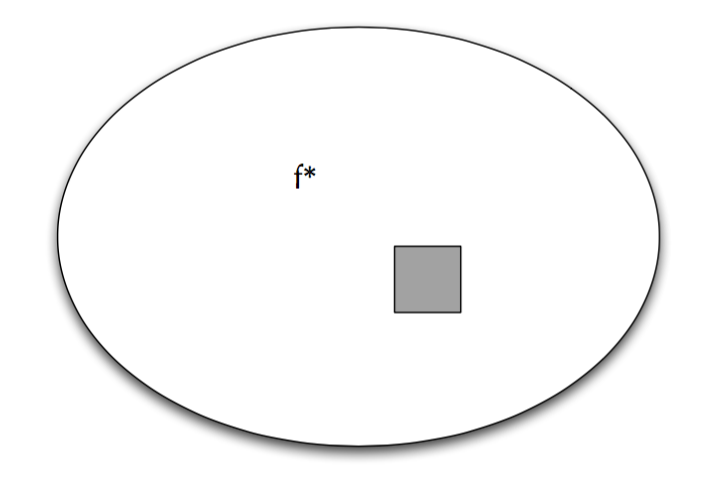
\includegraphics[width=0.8\textwidth]{f2}
\label{default}
\end{center}
\end{figure}

A parametric model is a small part of this space (the grey box)!


}

\frame{
\frametitle{Bayesian Nonparametrics}

\begin{figure}[htbp]
\begin{center}
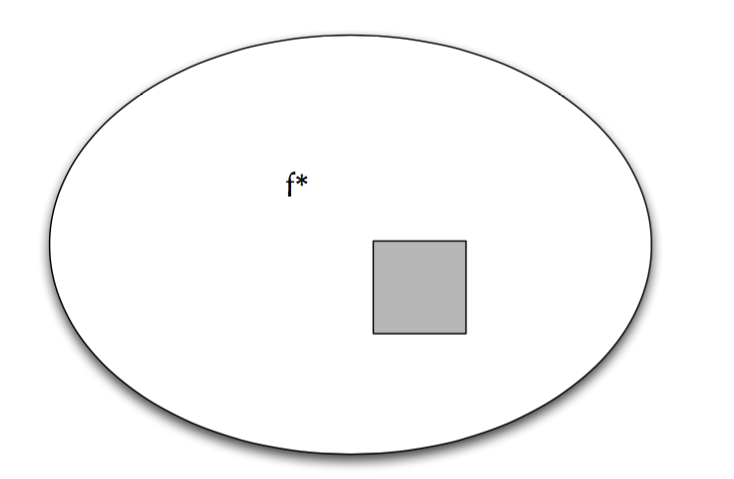
\includegraphics[width=0.8\textwidth]{f3}
\label{default}
\end{center}
\end{figure}
Let's increase the complexity of the model. 
Unlikely that true function will ever be in the parametric space. 

}


\frame{
\frametitle{Bayesian Nonparametrics}

\begin{figure}[htbp]
\begin{center}
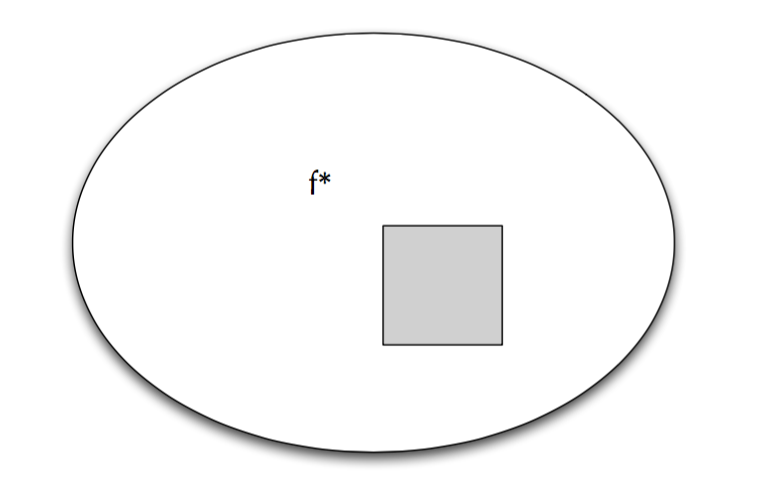
\includegraphics[width=0.8\textwidth]{f4}
\label{default}
\end{center}
\end{figure}
Let's increase the complexity of the model. 
Unlikely that true function will ever be in the parametric space. 

}

\frame{
\frametitle{Bayesian Nonparametrics}

\begin{figure}[htbp]
\begin{center}
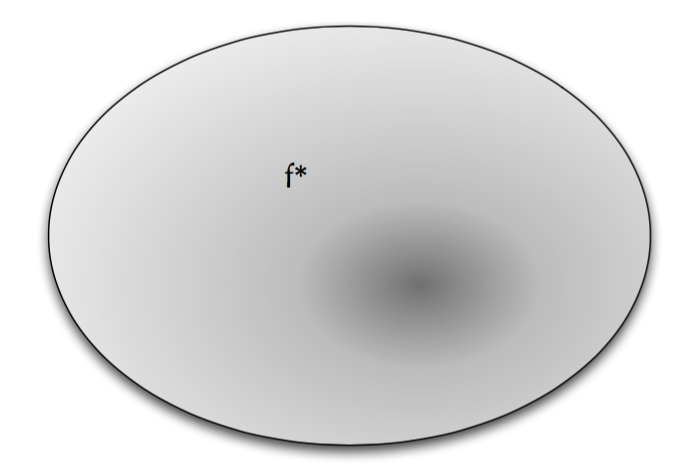
\includegraphics[width=0.8\textwidth]{fbnp}
\label{default}
\end{center}
\end{figure}
Instead, we look at a very reach space for efficient learning. Place higher probability for models that are likely and vice versa.

}

%\frame{
%\frametitle{BNP so far}
%
%What is the main advantage of BNP methods over parametric methods? 
%
%Give an example of a parametric model. What makes it parametric. 
%
%Give an example of a parametric model that could be considered nonparametric. Explain. 
%
%}







\frame{
\frametitle{What is the benefit of BNP?}

\begin{enumerate}
\item They work well for model selection and averaging. (We won't cover this).
\item They are good at fitting large functional spaces. 
\item They are good for structural learning. 
\end{enumerate}
}

\frame{
\frametitle{Are Nonparametric Models Nonparametric}
Nonparametric just means not parametric: cannot be described by a fixed set of parameters.

\vskip 1em

Nonparametric models still have parameters, they just have an infinite (very large) number of them.

%\vskip 1em
%
%Note: You can have a very giant parametric model that is in essence a BNP model. Why would this be true?

\vskip 1em

Nonparametric models still make modelling assumptions, they are just
less constrained than the typical parametric models.


}

\frame{
\frametitle{Issues with Bayesian Nonparametrics}

\begin{enumerate}
\item Developing classes of nonparametric priors suitable for modelling data.
\item Developing algorithms that can efficiently compute the posterior is important.
\item Developing theory of asymptotics in nonparametric models.
\end{enumerate}


}



\frame{

Goal: assign data points $x_1, \ldots x_n$ into clusters
$z_1, \ldots, z_K.$

\vskip 1em
What would be a good application or an example of our goal?

\begin{figure}[htbp]
\begin{center}
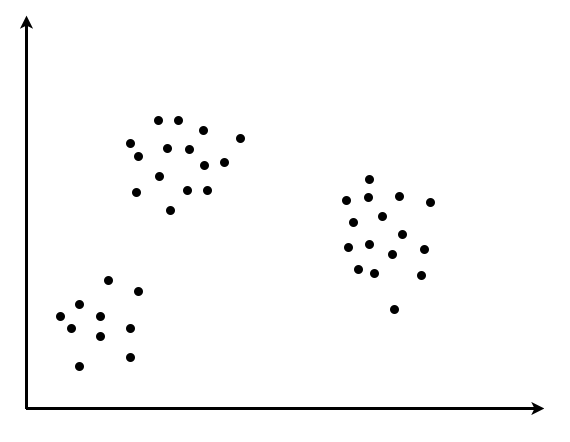
\includegraphics[width=0.5\textwidth]{clustering}
\caption{Suppose we have some data points that we want to cluster into groups.}
\label{default}
\end{center}
\end{figure}


}

\frame{
The data points could be classifying data points (pictures of animals) into 3 groups that are dog, cat, and mouse. 

\begin{figure}[htbp]
\begin{center}
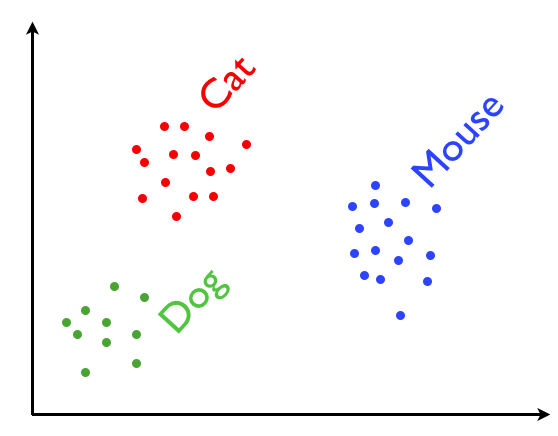
\includegraphics[width=0.5\textwidth]{clusteringExample}
%\caption{Suppose we have some data points that we want to cluster into groups.}
\label{default}
\end{center}
\end{figure}

For  another application, we might cluster students in a class into their majors: math, engineering, statistics, political science, environment, and economics.

}

\frame{

Example of what the cluster assignment of pictures (data points) to cat, dog, etc might look like. 

\begin{figure}[htbp]
\begin{center}
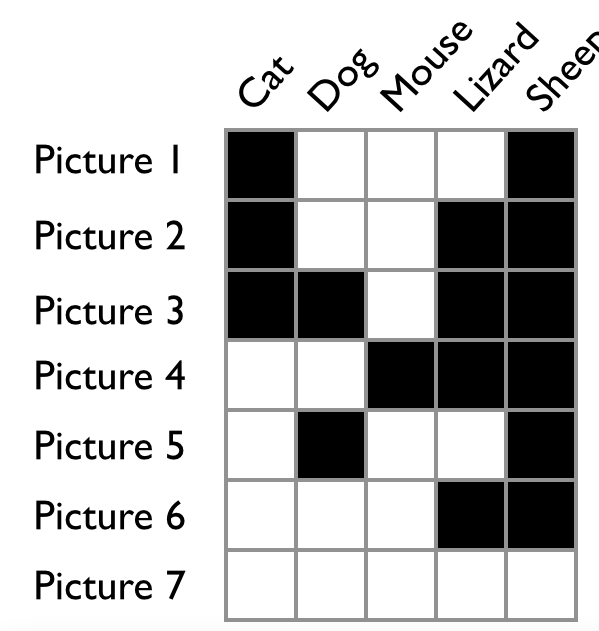
\includegraphics[width=0.5\textwidth]{latentFeature}
%\caption{Suppose we have some data points that we want to cluster into groups.}
\label{default}
\end{center}
\end{figure}



}

\frame{
\frametitle{Notation}
\begin{itemize}
\item $x_i, i=1,\ldots,n$: data points
\item $z_i, k=1\ldots,K$: cluster assignments
\item Note that $K$ and $n$ are fixed and known. 
\end{itemize}




}


\frame{
\frametitle{Finite Mixture Models}
For each data point $i$
\begin{align}
 z_i \mid  \pi &\sim \Multinomial(\pi) \\
 x_i \mid z_i, \theta_k* &\sim F(\theta_{z_i}*)
\end{align}
Mixing proportions
$$\pi = (\pi_1,\ldots \pi_k) \mid \alpha \sim \Dirichlet(\alpha/K,\ldots, \alpha/K)$$
\vskip 1em
Cluster k:
$$\theta_k\mid H \sim H$$

Remark: $\alpha$ is fixed and known. How to choose?
}

\frame{
\frametitle{Finite Mixture Models}
%Original paper: Rasmussen (2000). 

%\begin{enumerate}
%\item Assume a Bayesian mixture model. 
%\item Background: Multivariate methods, Dirichlet distribution, and the Normal-Inverse Wishart (N-IW). 
%\end{enumerate}

Indicator $z_i$ denotes which component (data point) $x_i$ belongs to. 

\begin{align}
 z_i \mid  \pi &\sim \Multinomial(\pi), k=1,\ldots,K \\
 x_i \mid z_i = k, \mu, \Sigma & \sim N(\mu_k, \Sigma_k), i=1,\ldots, n
\end{align}

Now let's introduce conjugate priors for the parameters:

\begin{align}
\pi  &\sim \Dirichlet(\alpha/K,\ldots, \alpha/K) \\
\mu_k, \Sigma_k & \sim H = \text{N-IW}(0,s,d,\phi), k=1,\ldots,K
\end{align}

[Rasmussen (2000)]
}

\frame{
\frametitle{Gibbs Sampling for Bayesian Mixture Models}
All conditional distributions are simple to compute.

\vskip 1em

Let $n_1(z)$ be the number of components (data points) assigned to cluster 1, etc.

\begin{align}
p(z_i = k\mid - ) &\propto \pi_kN(x_i; \mu_k, \Sigma_k),\\
\qquad \pi\mid z &\sim \Dirichlet(\alpha/K + n_1(z),\ldots, \alpha/K + n_K(z)),\\
\mu_k, \Sigma_k \mid  - \; &\sim \text{N-IW}(\nu',s',d',\phi')
\end{align}

Derivations are left as an exercise. 

\vskip 1em

A computational issue: This Gibbs sampler is not efficient. 

}

\frame{
\frametitle{Collapsed Gibbs Sampling}

The main idea is that we integrate out any variables that we don't need. 
\vskip 1em
We continue with a Gibbs sampling scheme and this speeds up computation. 
Let's integrate out $\pi, \mu, \Sigma.$ (Exercise).


Then 
\begin{align}
p(z_i = k\mid - ) &\propto 
\frac{
\alpha/K + n_k(z_{-i})
}
{\alpha +n -1}
\times p (x_i \mid 
x^{(-i)}, n_k(z_{-i}))
\end{align}

Interpretation of the three pieces above:
\begin{enumerate}
\item $\alpha/K$: A pseudo count.
\item $n_k(z_{-i})$: Count up the number of times cluster $k$ was chosen among all the others except the $i$th. 
\item $\alpha +n -1$: The normalizing constant! 
\end{enumerate}

}

\frame{
\frametitle{Infinite Mixture Models}
\begin{enumerate}
\item We will take $K \rightarrow \infty.$
\item There are at most $n < K$ occupied components, so most components are empty. We can lump
these empty components together. 
%\item Note: This type of a model and approach works for most types of clustering tasks. Think at home when it would fail. 
\end{enumerate}
%
\textcolor{blue}{Occupied components}:
\begin{align}
p(z_i = k \mid -) 
&\propto 
\frac{
\alpha/K + n_k(z_{-i})
}
{\alpha +n -1}
\times p (x_i \mid x_k^{-i})
\end{align}
For clusters that are occupied  ($n_k > 0$), things are well defined. 

\vskip 1 em

Let K* = the empty clusters and $\{\}$ denotes an empty component. 

\textcolor{blue}{Empty components}:
\begin{align}
p(z_i = k_{empty} \mid z^{-i}) 
&\propto 
\frac{
\alpha \times \frac{(K-K*)}{K}
}
{\alpha +n -1}
\times p (x_i \mid \{\})
\end{align}





}

\frame{
\frametitle{Infinite Mixture Models}
Now let $K\rightarrow \infty.$
\vskip 1em
 
\textcolor{blue}{Occupied components}:
\begin{align}
p(z_i = k \mid -)  &\propto 
 n_k(z_{-i})
\times p (x_i \mid x_k^{-i})
\end{align}


\vskip 1 em


\textcolor{blue}{Empty components}:
\begin{align}
p(z_i = k_{empty} \mid z^{-i}) 
&\propto 
\alpha \times p (x_i \mid \{\})
\end{align}

}

\frame{
\frametitle{But wait -- this makes zero sense in general!}

\begin{itemize}
\item The actual infinite limit of finite mixture models does not make sense: any particular component will
get a mixing component of zero. 
\item In the Gibbs sampler, we got around this by lumping empty clusters together. 
\item Other ways of making this limit precise:
\begin{itemize}
\item Looking at the prior clustering structure induced by the Dirichlet prior over mixing proportion---Chinese restaurant process. 
\item Re-order components so that those with larger mixing proportions tend to occur first, before taking the limit--stick-breaking construction. 
\end{itemize}
\item Both are different views of the Dirichlet process (DP).
\item DPs: can be thought of infinite dimensional Dirichlet distributions. 
\item The $K\rightarrow \infty$ Gibbs sampler is for DP mixture models.


\end{itemize}



}

\frame{
\frametitle{A Tiny Bit of Measure Theory}
In order to formally define some upcoming terms, we need to understand a measure.
\vskip 1em

Informally, a measure is like a ruler! 

\vskip 1em

On the real line, the measure is the length of a subset of the real line. 


\vskip 1em

We typically can't work with the entire real line and must work with subsets (or families
of subsets). [This is known as a $\sigma$-algebra]

\vskip 1em

Then due to this, we will have some properties so that we can apply our measure or ruler. 


}

\frame{
\frametitle{A Tiny Bit of Measure Theory}
\begin{itemize}
\item A $\sigma$-algebra $\Sigma$ is a family of subset of a set $\Theta$ such that
\begin{itemize}
\item $\Sigma$ is not empty (\textcolor{red}{we can measure something}).
\item If $A \in \Sigma$ \textcolor{red}{measurable set}, the $\Theta \setminus A \in \Sigma$
\item If $A_1,A_2,\ldots \in \Sigma$ then $\cup_{i=1}^{\infty} A_i \in \Sigma.$
\end{itemize}
\item $(\Theta, \Sigma)$ is a measure space and $A \in \Sigma$ are the measurable sets.
\item A measure $\mu$ over $(\Theta, \Sigma)$  is a function $\mu: \Sigma \rightarrow [0,\infty]$ such that
\begin{itemize}
\item $\mu(\emptyset) = 0.$
\item If $A_1,A_2,\ldots \in \Sigma$ are disjoint then $\mu(\cup_{i=1}^{\infty} A_i) = \sum_{i=1}^{\infty} \mu(A_i)$
\item Everything that we consider will be measurable
\item A probability measure is one where $\mu(\Theta) = 1.$
\end{itemize}
\end{itemize}

}

%\frame{
%\frametitle{A Tiny Bit of Measure Theoretic Probability Theory}
%
%If $p$ is a probability measure on $(\Theta, \Sigma)$, then a random variable $X$ taking values in $\alpha$ is simply a measurable function $X: \Theta \rightarrow \alpha.$
%
%\begin{itemize}
%\item Think of the probability space $(\Theta, \Sigma, \rho)$ as a black-box random number generator 
%\item and $X$ as a function
%taking random samples in $\Theta$ and producing random samples in $\alpha.$
%\end{itemize}
%
%\vskip 1 em
%
%What's really going on here? 
%
%\vskip 1 em
%
%A random variable isn't actually random. It's just a measurable function (fixed). 
%
%\vskip 1 em
%
%How would you implement a function to generate random draws from a Normal(10,1)?
%(The only thing at your disposal is a random number generator). 
%
%%\vskip 1 em
%%
%%\begin{enumerate}
%%\item Assume a random number generator. (Deterministic) 
%%\item This random number generator will generate a standard normal
%%\item Now add 10 to it. 
%%\end{enumerate}
%%Repeat to get N sample points. 
%
%}
%
%\frame{
%\frametitle{Stochastic processes}
%
%A stochastic process is a collection of random variables $\{X_i\}_{i\in I}$ over the same measurable space $(\Theta, \Sigma)$, where $I$ is an index set.
%
%\begin{itemize}
%\item Stochastic processes are different from other models as that they can be infinite (even uncountably so). 
%\item This raises issues of how do you even define them and how to do you ensure they exist (mathematically speaking). 
%\end{itemize}
%
%Stochastic processes form the core of many Bayesian nonparametric models, so they will be useful. 
%
%}

%\frame{
%\frametitle{The k-simplex}
%
%What is a k-simplex? (Formally, we will define it). 
%
%\vskip 1 em
%
%When k=2, the simplex is a line. 
%
%\vskip 1 em
%
%When k=3, the simplex is a triangle.
%
%\vskip 1 em
%
%In general, the simplex is a type of polytope. 
%
%
%}

\frame{
\frametitle{Dirichlet Distribution}

A Dirichlet distribution is a distribution of the $K$-dimensional probability simplex
$$\bigtriangleup_K = \{(\pi_1,\ldots, \pi_k): \pi_k \geq 0, \sum_k \pi_k = 1\}$$

We say that $(\pi_1,\ldots, \pi_k)$ is Dirichlet distributed:

$$(\pi_1,\ldots, \pi_k)\sim \text{Dir}(\alpha_1,\ldots,\alpha_k)$$
if
$$p(\pi_1,\ldots, \pi_k) = \frac{\Gamma(\sum_k \alpha_k)}
{\prod_k \Gamma(\alpha_k)} 
\prod_{k=1}^K \pi_k^{\alpha_{k-1}}$$


}


\frame{

\begin{figure}[htbp]
\begin{center}
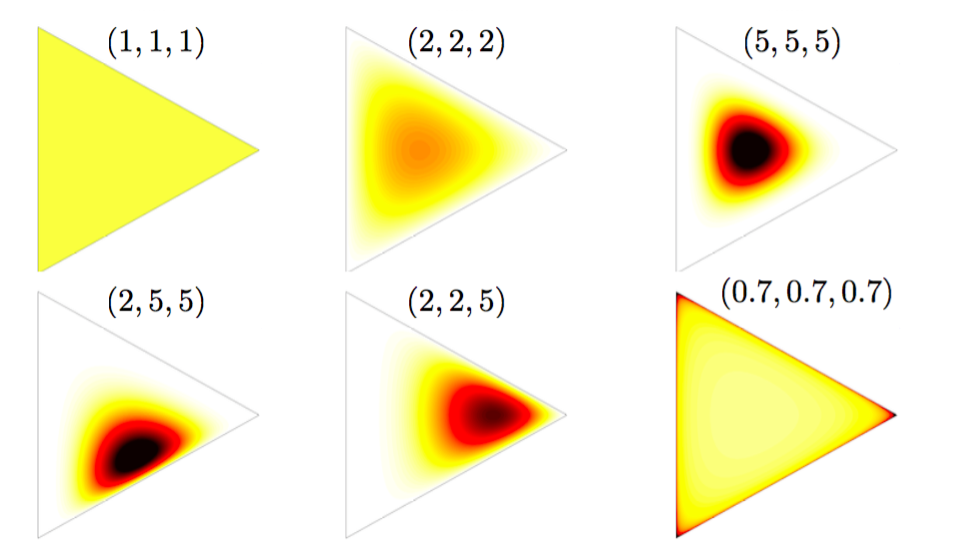
\includegraphics[width=0.9\textwidth]{dir}
\caption{Far left: We get a uniform prior on the simplex. Moving to the right we get things unimodal. On the bottom, we get distributions that are multimodal at the corners.}
\label{default}
\end{center}
\end{figure}



}

\frame{
\frametitle{Dirichlet Process}


\vskip 1em

A Dirichlet Process (DP) is a randomly probability measure $G$ over 
$(\Theta, \Sigma)$ such that for any finite set of measurable partitions
$A_1 \cup \cdots \cup A_k = \Theta,$ we have 

\begin{align}
(G(A_1)), \ldots, G(A_k)) \sim \text{Dir}(\alpha H(A_1), \ldots, \alpha H (A_k))
\end{align}
where $\alpha$ is the concentration parameter and $H$ is the base measure. 


\begin{figure}[htbp]
\begin{center}
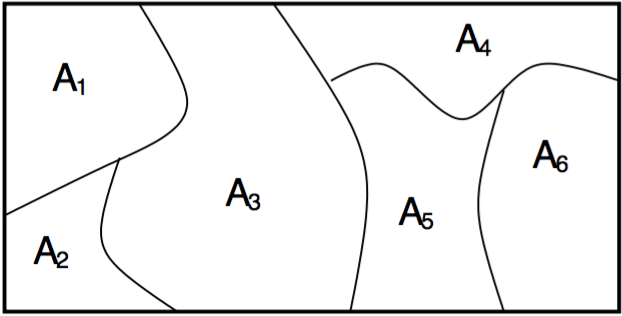
\includegraphics[width=0.6\textwidth]{partitions}
\label{default}
\end{center}
\end{figure}

[Ferguson, 1973], Formal definition, Not constructive.

}

\frame{
\frametitle{Parameters of the DP}

\begin{itemize}

\item $\alpha$ is the concentration, strength, or mass parameter.
\item $H$ is the base measure or distribution. 
\item Mean and variance:
$$E[G(A)] = H(A)$$
$$ V(G(A)) = \frac{H(A) (1-H(A))}{\alpha+1}.$$
where $A$ is a measurable subset of $\Theta.$
\end{itemize}

\vskip 1em
Exercise: Derive the mean and variance. 

}

\frame{
\frametitle{Dirichlet Process}
A Dirichlet Process is a distribution over distributions. 
Suppose $$G \sim DP(\alpha, H)$$
$$x_i \mid G \sim G, i=1,\ldots,N$$ (iid given G)

\vskip 1em
The Dirichlet-Multinomial conjugacy carries over to the DP:

$$G \mid x_1,\ldots,x_{n-1} \sim 
DP(\alpha + n, \frac{\alpha H + \sum_i \delta_{x_i}}{\alpha + n-1})$$

\vskip 1em
Exercise: Verify that conjugacy holds.
% $$P(\bm{X}) = \int P(G) \prod_{n=1}^N P(X_n \mid G) dG.$$

}



\frame{
\frametitle{Polya Urn Scheme}
\begin{align}
G &\sim DP(\alpha, H)\\
x_i &\mid G \sim G \quad \text{for all} \; n
\end{align}
\vskip 1em
Marginalizing out G we get
$$x_{n} \mid x_1,\ldots, x_{n-1} \sim \frac{\alpha H +\sum_i \delta_{x_i}}
{\alpha + n-1}$$

This is equivalent to 
$$
x_{n} \mid x_1,\ldots, x_{n-1} =
\begin{cases}
x_i^* & \text{with prob} \; \dfrac{c_n(x_i)}
{\alpha + n -1} \\
\text{new draw from H} &\text{with prob} \; \dfrac{\alpha}
{\alpha + n -1} \\
\end{cases}
$$
where $c_n(x_i)$: number of customer at table $i$ when customer $n$ makes a move. 

%You can show this since $$P(\bm{X}) = \int P(G) \prod_{n=1}^N P(X_n \mid G) dG.$$

}

\frame{
\textcolor{blue}{
Marginalizing out G we get
$$x_{n} \mid x_1,\ldots, x_{n-1} \sim \frac{\alpha H +\sum_i \delta_{x_i}}
{\alpha + n -1 }$$
}

is called the Polya urn scheme. 
\vskip 1em

Assume that G is a distribution over colors and each $X_n$ represents the color of a single ball placed in the urn. 

\begin{figure}[htbp]
\begin{center}
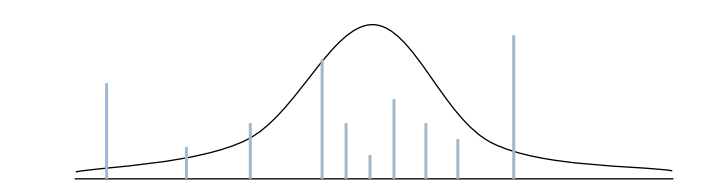
\includegraphics[width=0.7\textwidth]{polya}
\label{default}
\end{center}
\end{figure}
}

\frame{

\textcolor{blue}{
Marginalizing out G we get
$$x_{n} \mid x_1,\ldots, x_{n-1} \sim \frac{\alpha H +\sum_i \delta_{x_i}}
{\alpha + n -1}$$
}

Start with an empty urn. On step $i$:
\begin{enumerate}
\item With probability proportional to $\alpha$, draw $X_n \sim H$ and add a ball of that color to the urn.
\item With probability proportional to $n-1$ (number of balls currently in the urn), pick a ball at random from the urn. 
\begin{enumerate}
\item Record it's color as $X_n$ and return its ball into the urn, along with a new one of the same color.
\end{enumerate}
\end{enumerate}
Repeat for $i=1,\ldots {N}$



%\begin{itemize}
%\item Have an urn with $\alpha$ balls of color \textcolor{red}{red}.
%\item Pick a ball randomly from the urn.
%\item If the urn has color \textcolor{red}{red}, make a new ball with the color sampled from H. Note the color; return both balls to the urn.
%\item If the urn does not have the color \textcolor{red}{red}, return two \textcolor{red}{red} balls to the run. 
%\end{itemize}

[Blackwell \& MacQueen 1973, Hoppe 1984]
}

\frame{
\frametitle{Stick Breaking Construction of the DP}
In 1994, Sethuraman developed a constructive way of G, called the ``stick breaking" construction. 
\vskip 1em
First assume we have a stick of length 1 (or unit length). 
\vskip 1em
At each iteration, we break part of the stick of with probability $\pi_i$. 
\vskip 1em
The proportion remaining at each iteration is $\mu_i.$

\begin{figure}[htbp]
\begin{center}
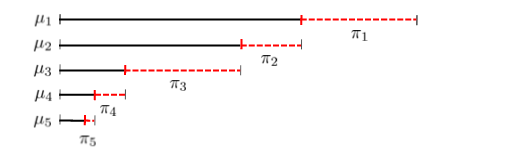
\includegraphics[width=\textwidth]{stick}
\label{default}
\end{center}
\end{figure}

}

\frame{
$V_i$ is proportion to cut at iteration $i.$
The remaining length is then 
$$\prod_{j=1}^{i-1}(1-V_j)$$
And the broken part is 
$$\pi_i(\bm{v}) = V_i \prod_{j=1}^{i-1}(1-V_j).$$

Let's assume that $$V_i \sim \Beta(1,\alpha)$$
}

\frame{
\begin{align}
G &= \sum_{i=1}^\infty \pi_i(\bm{v}) \delta_{X_i}\\
V_i, &\sim \Beta(1, \alpha)\\
X_i & \sim H\\
f(V_i =v_i \mid \alpha) & = \alpha (1-v_i)^{\alpha-1}\\
\pi_i(\bm{v}) &= V_i \prod_{j=1}^{i-1}(1-V_j)
\end{align}

}

\frame{
\frametitle{Finite Mixtures}
This ties back into Finite Mixture Models and Infinite Mixture Models

\begin{figure}[htbp]
\begin{center}
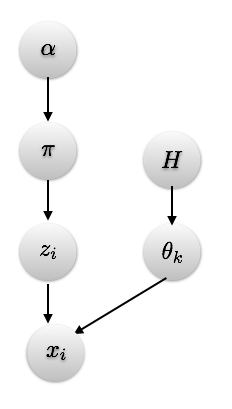
\includegraphics[width=0.3\textwidth]{finiteMixture}
\label{default}
\end{center}
\end{figure}

%\begin{align}
%
%
%\end{align}


}

\frame{
\frametitle{DP Mixtures}
\begin{align}
G\mid \alpha, H &\sim DP(\alpha,H) \\
\theta_i &\mid G\sim G \\
x_i \mid \theta_i &\sim F(\theta_i)
\end{align}
\begin{itemize}
\item $\theta_i$ are clustered according to a Polya urn scheme
\item Other representation is via by the stick breaking representation. 
\end{itemize}

\begin{figure}[htbp]
\begin{center}
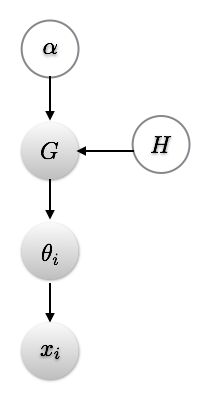
\includegraphics[width=0.2\textwidth]{dpMixture}
\label{default}
\end{center}
\end{figure}

}

\frame{
\begin{itemize}
\item Formalize representations for the CRP and Stick breaking. 
\item There are many other extensions of a DP. 
\item In lab and in homework you will go through the CRP.
\item Remember that the CRP and Stick breaking are special cases of the DP. 
\item We did not have time to cover inference, but I'm happy to point you to references, etc if you want to read more. 
\end{itemize}



}



%\frame{
%
%Now show what a simulation looks like. 
%Then do stick breaking. End the class. 
%
%
%
%}
%
%
%
%\frame{
%\frametitle{Clustering Property}
%\begin{align}
%G &\sim DP(\alpha, H)\\
%x_i &\mid G \sim G \quad \text{for all} \; i
%\end{align}
%\vskip 1em
%
%The variables $x_1, x_2, \ldots, x_n$ can take on $K \leq n$ distinct values. 
%
%\begin{itemize}
%\item Let the distinct values be $x_1*, \ldots, x_k*.$ This defines a partition of $\{1,\ldots,n\}$ such that $i$ is in cluster $k$ if and only if $x_i = x_k^*.$
%\item The induced distribution over partitions is the Chinese restaurant process (CRP). 
%\end{itemize}
%
%
%
%
%}
%
%
%
%\frame{
%\frametitle{Partitions}
%
%A partition $\eta$ of a set S is 
%\begin{itemize}
%\item A disjoint family of non-empty subsets of S whose union is S.
%\item $S = \{Alice, Bob, Charles, David, Emma, Florence \}$
%\item $\eta = \{ \{Alice, David\}, \{Bob, Charles, Emma\}, \{Florence\}$
%\}
%\end{itemize}
%
%\begin{figure}[htbp]
%\begin{center}
%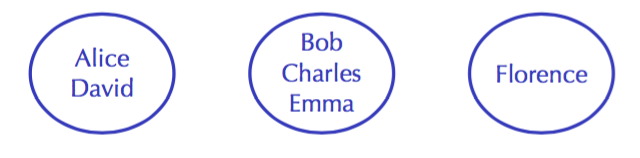
\includegraphics[width=0.6\textwidth]{alice}
%\label{default}
%\end{center}
%\end{figure}
%
%Denote the set of all partitions of S as $\mathcal{P}_S.$
%\vskip 1em
%
%Random partitions are random variables taking values in $\mathcal{P}_S.$
%\vskip 1em
%We will work with partitions of $S = [N] =\{1,2,\ldots,N\}.$
%
%
%}
%
%\frame{
%\frametitle{CRP}
%
%
%
%\begin{figure}[htbp]
%\begin{center}
%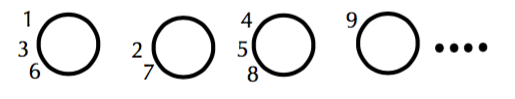
\includegraphics[width=0.6\textwidth]{crp}
%\label{default}
%\end{center}
%\end{figure}
%
%$n_c =$ number of people at table $c$; $\alpha>0.$
%\begin{itemize}
%\item Each customer comes into restaurant and sits at a table:
%$$p(\text{sit at table c}) = \frac{n_c}{\alpha + \sum_{c\in \eta} n_c} =   \frac{n_c}{\alpha + n - 1} $$ and
%$$p(\text{sit at new table}) = \frac{\alpha}{\alpha + \sum_{c\in \eta} n_c}= \frac{\alpha}{\alpha + n -1}$$
%\item Customers correspond to elements of $S,$ and tables to clusters in $\eta$.
%\item Richer get richer process: large clusters are more likely to attract more customers. 
%\end{itemize}
%
%[Aldous 1985, Pitman 2006]
%}
%
%\frame{
%\frametitle{Model Based Clustering}
%How can we use the CRP in model based clustering? 
%\vskip 1em
%For every cluster $c$ in our partition $C$ is to introduce a prior over partitions. 
%\vskip 1em
%A CRP can be nice for modeling a prior over partitions. 
%\begin{itemize}
%\item Can derive the finite mixture model from this model.
%\item To do this directly, we derive a finite mixture model
%\end{itemize} 
%
% 
%
%
%}
%
%\frame{
%\frametitle{Finite Mixture Model}
%
%Suppose there are potentially $K$ clusters. 
%\begin{itemize}
%\item Each cluster $k$ has parameter $\theta_k$
%\item Each data point $i$ assigned to $k$ has mixing probability $\pi_k$
%\end{itemize} 
%This induces a random partition with at most $K$ clusters. 
%\vskip 1em
%
%For the priors on the other parameters:
%
%\begin{align}
%\pi \mid \alpha &\sim \Dirichlet(\alpha/K,\ldots,\alpha/K)\\
%\theta_k^* \mid H &\sim H
%\end{align}
%
%
%
%}
%
%\frame{
%
%
%What is the induced distribution over partitions? 
%
%}

\end{document}